\documentclass{article}
\author{Wenzhao Xu (Environmental Engineering)\\ Haoyan Cai (Statistics)}
\title{STAT 542 Mid Report}
\usepackage{amsmath}
\usepackage{graphicx}
\usepackage{subfig}
\usepackage{multirow}
\usepackage[top=1in, bottom=1in, left=1.25in, right=1.25in]{geometry}


\begin{document}
	\maketitle
	
	\section{Introduction} % (fold)
	\label{sec:introduction}
	\paragraph{} The data are about accelerometer data from mobile devices. The train data contain X,Y,Z axis acceleration values from 387 devices and testing data set consists of 90024 testing sequences. Each test sequence comes with a proposed device Id. The goal is to judge whether the claimed device is the true device that produces the test sequence. The main difficulties in this project are: (1) Data has outliers and gaps (i.e. the sampling time interval is not constant so that two sampling points might have very large time interval); (2) Feature extractions; (3) Treat it as a multi-label classification problem or as a 0-1 classification problem by some label creating methods. 
	
	% section introduction (end)
	
	\section{Method} % (fold)
	\label{sec:method}
	\paragraph{} The basic assumption is that each user will behavior similar if he/she is doing the same activity and he/she would probabily do the same activity at the same time of day. 
	\paragraph{}First we treat it as a multi-label problems, that is trying to predict which device generates the test sequence. Given the training data of a certain device, we first divided the whole training data into pieces, each has around 400 points (400 is a tuning parameters). For most devices, 400 sampling points will last for about 1 minute and we assume the user is doing the same activities in this 1 minute. Each piece represents an activity, no matter what the activity is. So for train data of a device, we have several pieces and all of them have the same label as that device ID. Features are extracted from these pieces and also from the test sequences. In this way, we have training sequences with labels and test sequences. Certain classifier is trained and predicted the labels of test sequences.
	\paragraph{} We also tried to change the problem as a 0-1 classification problem. XXXXX, currently, we are still working on it. 
	
		\subsection{Data Preparation} % (fold)
		\label{sub:idea}
		\paragraph{} The data is imported into R by "ff" packages (SQL database technique is also available). Then the data is preprocessed through splitting,resampling and smoothing to get the final training data and test data. Figure 1 shows an brief of how data is pre-processed.
		
		\begin{figure}
			\centering
			\subfloat[Splitting]{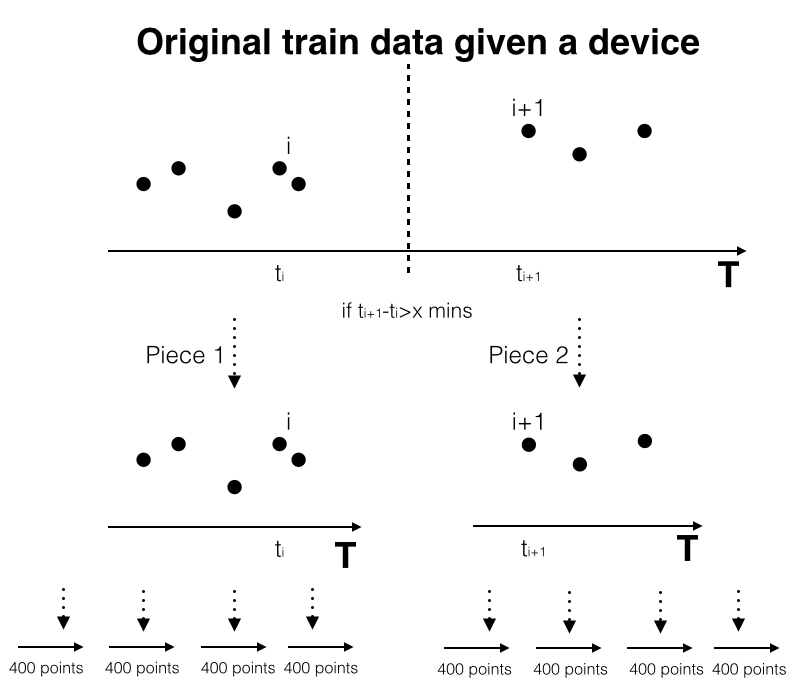
\includegraphics[width=0.6\textwidth]{split.png}}
			\subfloat[Resampling]{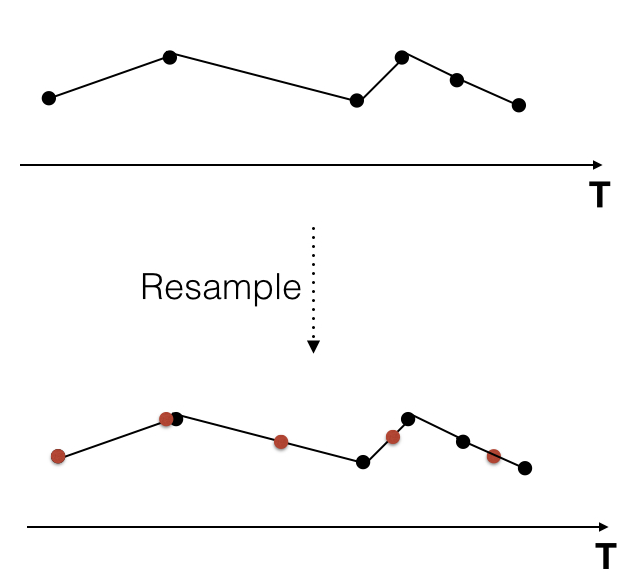
\includegraphics[width=0.4\textwidth]{resampling.png}}
			\caption{Splitting and Resampling Steps}
		\end{figure}
		
		
		
		 \subsubsection{Splitting}
		\paragraph{}It is found that the training data of a given device don't have a constant sampling frequency, that is, the time interval of sampling poitns are not the same. This might be due to users' manually switching off device or the way Android OS deal with accelerometer sensors. So the whole training data might have large gaps in time. In order to deal with this, we first calcuate the sampling time intervals. If the time interval is larger that 2 minutes, we split the training data into two data pieces at this point. After the data is divided into several pieces, we further divide each pieces into smaller sequences, each sequence has 400 raw data points. At the end of this step, the training data from 387 devices are splited into almost 70000 sequences. This step is shown in Figure 1(a).
		In addition, for test data, similar splitting method is used. If the time interval in one test sequence is larege than 3 minutes, we divide the test sequence into 2 parts and discard the part with less data points. 
		\subsubsection{Resampling}
		\paragraph{} In splitting step, we split the train data into sequences. However, in each sequence, the sampling frequencies are not always the same. Some might be 200 ms other others might be around 100ms.  Such inconsistance makes it very hard for further analysis, especially for frequency analysis. So we do a resample step. A constant sampling time is set based on the initial sampling time and the median value of original sampling intervals. Here median value is used to eliminate the influence of sampling interval outliers. Then, on the new sampling time, the resampled acceralation value is calculated by linear interpolation based on two nearest sampling points. In Figure 1(b), the brown points are the new data points based on interpolation. 
		\subsubsection{Smoothing}
		\paragraph{} Train data have noises such as large spikes. So a 5-point moving average algorithm is then used to smooth the data. 5-point moving average is also used in other literatures. Figure 2 shows the data piece before and after resampling and smoothing steps.
		% subsection idea (end)
		\begin{figure}
			\centering
			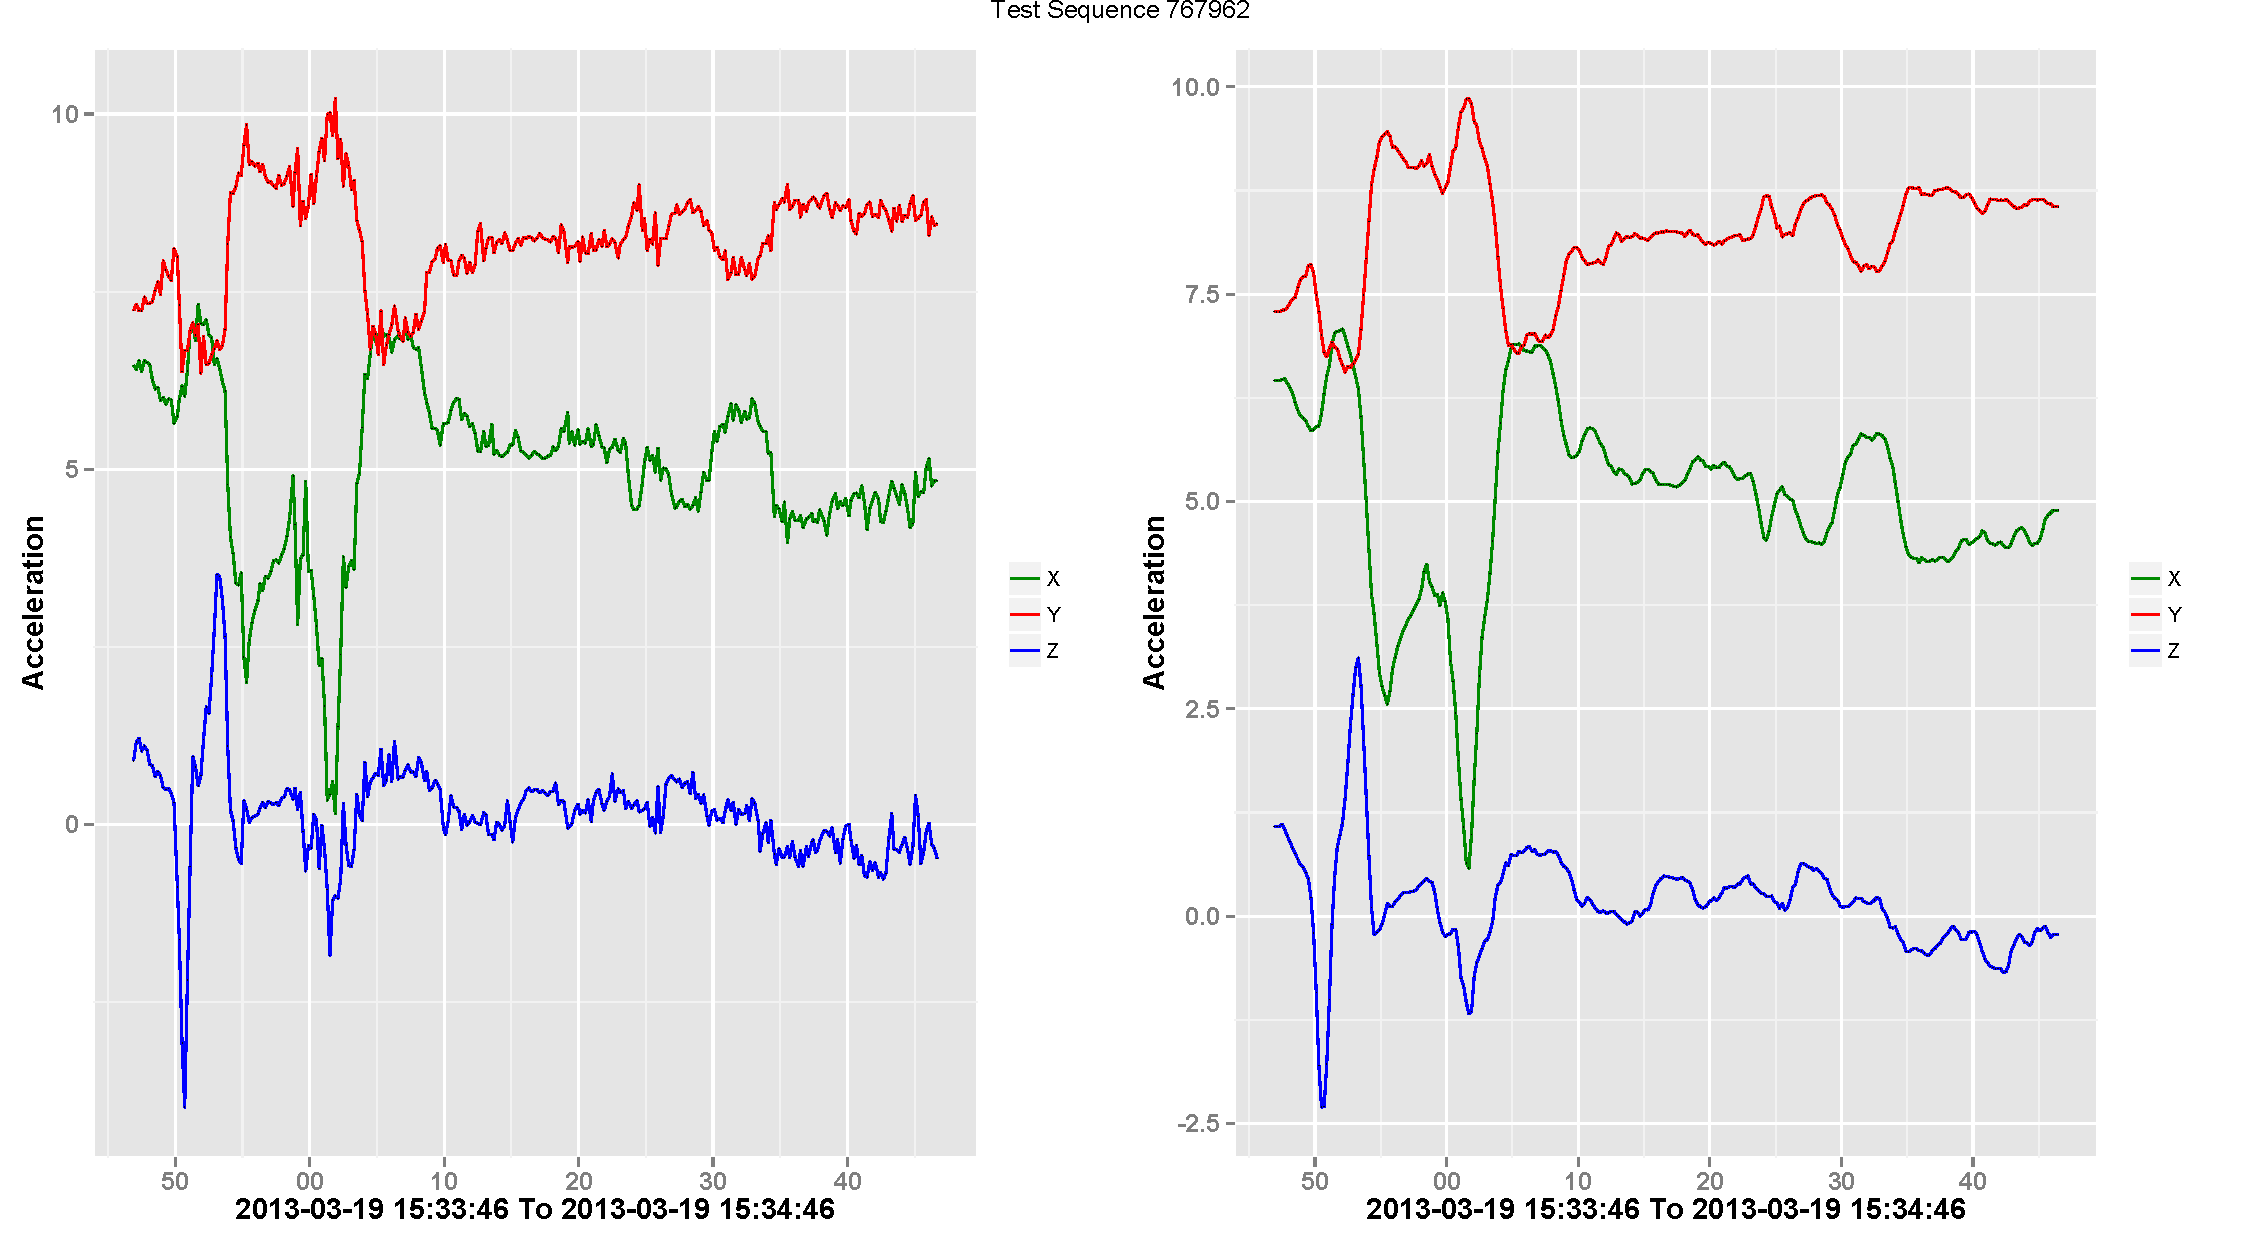
\includegraphics[width=0.9\textwidth]{Rplot.pdf}
			\caption{Comparison before and after resampling and smoothing}
		\end{figure}
	
	
		\subsection{Feature Extraction} % (fold)
		\label{sub:feature_extraction}
		
		\paragraph{}First, the total acceralation value is calculated by $A=\sqrt{(a_x^2+a_y^2+a_z^2)}$ and added as a new time series. Based on literature research, 4 kind of features are extracted from the raw data. The first is mean and variance. The second is the correlation. The third is the frequency pattern and the last is the time. Totally, the number of features are 20, which is shown in Table 1. 
		\begin{table}
			\centering
			\caption{Feature Selection}
			\begin{tabular}{p{3cm}|p{6cm}|p{4cm}}
			Kind & Description & Physical Meanings \\ \hline
			1.Mean and Variance (8 features) & Mean and variance of acceleration values in each axis as well as the total accerlation $A$ & The habbit of how user put their cellphones and the strength of their activities \\ \hline
			2.Correlation (cor) (3 features) & the correlation coefficients between x and y, x and z, and y and z axis. & The users features when doing activities \\ \hline
			3.Frequency Features (8 features) & The mean value of the first 5 dominate frequencies (frequencies with highest amplitude) and mean value of energy in these frequencies & Users walking features.\\ \hline
			4.Time (1 feature) & mean time of day & User's habbit when doing such activity.
			\end{tabular}
		\end{table}

		% subsection feature_extraction (end)
	
		\subsection{Classifier} % (fold)
		\label{sub:classifier}
		\paragraph{} For simplicity, currently we just use KNN methods to detemine which device generate the test sequence. This is a multi-label classification problem, so other available methods include random forest and regression. 
		
		\paragraph{} However, if we treat the problem as a bi-label problem, other method such as SVM is also available. XXXXX
		% subsection classifier (end)
	% section method (end)
	
	\section{Result} % (fold)
	\label{sec:result}
	\paragraph{} The data preparation and feature extraction took about 20 mins from training data and 34 mins for test data. For simplicity, KNN is first used to predict the test sequences. The features are first scaled and we all the features except the time features. The result is uploaded to the kaggle website to see the result. We do some initial features selection and the result is shown in Table 2. 
	\begin{table}
		\centering
		\caption{Prediction Result}
		\begin{tabular}{c|c|c|c}
			Feature Selection & Num of Features & Score & Rank \\ \hline
			Kind 1,2 & 11 & 0.49995 & 621 \\ 
			Kind 1,2,3 & 19 & 0.61843 & 481 \\ 
			Kind 1,2,3,4 & 20 & 0.5 & 619 \\
		\end{tabular}
	\end{table}
	The best is with score as 61.843 and rank as 481, which is better than the KNN benchmark. Full features does't perform which indicates the users might not behavior similar in the same day of time or the weights of features need more analysis. In addition, frequency features are very important to improve the performance. 
	
	
	% section result (end)
	
	\section{Future Work} % (fold)
	\label{sec:future_work}
	\paragraph{} We plan to take a better analysis on feature extraction, and also take smaller or larger training pieces to see the change of results. Moreover, other method such as random forest and ANN will be applied to see the improvment. Finally, features selections will also be performed. 
	% section future_work (end)
	
\end{document}